% !TEX root = main.tex
\section{Time dependent amplitude fit}
\label{sec:fullFit}


\subsection{Signal Model Construction}
\label{sec:LASSO}

The light meson spectrum comprises multiple resonances which are expected to contribute to $B_s \to D_s K \pi \pi$  decays as intermediate states. 
Apart from clear contributions coming from resonances such as $K_{1}(1270)$, $K_{1}(1400)$ $\rho(770)$ and $K^*(892)^0$, 
the remaining structure is impossible to infer due to
the cornucopia of broad, overlapping and interfering resonances 
within the phase space boundary.
The complete list of considered amplitudes can be found in Appendix \ref{a:decays}.

To build the amplitude model, one could successively add amplitudes on top of one another until a reasonable agreement between data and fit was achieved.
However, this step-wise approach is not particularly suitable for amplitude analyses as discussed in Ref.~\cite{Guegan:2015mea}.
%In practice, this sum has to be truncated at some point.
%It is clear that adding more fit parameters will 
%describe our data better
%but including too many degrees of freedom leads to overfitting,
%\ie reduces predictive power and
Instead, we include the whole pool of amplitudes in the first instance and use the 
Least Absolute Shrinkage and Selection Operator~\cite{Tibshirani94regressionshrinkage,Guegan:2015mea} (LASSO) approach to limit the model complexity.
%, as proposed in Ref.~\cite{Guegan:2015mea}. 
% in the context of amplitude analyses.
In this method, the event likelihood is extended by a penalty term
\begin{equation}
	-2 \, \log \mathcal L \to -2 \, \log \mathcal L + \lambda \, \sum_{i} \sqrt{ \int \vert a_{i} \, A_{i}(\phsPoint) \vert^{2} \, \text{d}\Phi_{4}  },
\end{equation}
which 
%regularizes the amplitude coefficients.
%The imposed constraint on the 
%which limits the model complexity. 
% penalizing the absolute values of the
%coecients introduces shrinkage towards zero
%This constrained optimization 
shrinks the amplitude coefficients
%estimated parameters 
towards zero.
The amount of shrinkage is controlled by the parameter $\lambda$, to be tuned on data.
Higher values for $\lambda$ encourage sparse models, \ie models with only a few non-zero amplitude coefficients.
%Scanning over possible $\lambda$ values results in a ensemble of models with different 
The optimal value for $\lambda$ is found by minimizing the Bayesian information criteria~\cite{BIC} (BIC),
\begin{equation}
	\text{BIC}(\lambda) = - 2 \, \log \mathcal L + r  \, \log N_{\rm Sig},
\end{equation}
where $N_{\rm Sig}$ is the number of signal events and $r$ is the number of amplitudes with a decay fraction above 
a certain threshold.
In this way, the optimal $\lambda$ balances
the fit quality ($- 2 \, \log  \mathcal L$) against the model complexity.
The LASSO penalty term is only used to select the model. 
Afterwards, this term must be discarded in the final amplitude fit with the selected model, otherwise the parameter uncertainties would be biased. 

The set of amplitudes is selected using the optimal value of $\lambda=28$, and is henceforth called the LASSO model; 
Figure \ref{fig:BIC}(a) shows the distribution of BIC values obtained by scanning over $\lambda$
where we choose the decay fraction threshold to be $0.5 \%$.
In addition, we repeated the model selection procedure under multiple different conditions:
\begin{enumerate}
	\item The fit fraction threshold for inclusion in the final model was varied within the interval $[0.05, 5] \%$.
		The set of selected amplitudes is stable for thresholds between $0.1\%$ and $1\%$. 
		Other choices result in marginally different models containing one component more or less.
	\item Instead of BIC, the Akaike information criteria ($\text{AIC}(\lambda) = -2 \, \log  \mathcal L + 2 \, r$ \cite{AIC}) was used to optimize $\lambda$.
		For a given threshold, the AIC method tends to prefer %slightly 
		lower $\lambda$ values.
		However, the set of models obtained varying the threshold within the interval $[0.05, 5] \%$
		is identical to the BIC method. 
	\item The amplitudes selected under nominal conditions were excluded one-by-one from the set of all amplitudes considered.  
\end{enumerate}
From that we obtained a set of alternative models shown in Appendix~\ref{a:alternative}.

%\begin{figure}[b]
%  \centering
%  \includegraphics[width=0.49\textwidth, height=!]{figs/BIC_4pi.eps} 
%  \includegraphics[width=0.49\linewidth, height=!]{figs/BIC_KKpipi.eps}
%  \caption{Difference in the BIC value from its minimum as function of the LASSO parameter $\lambda$ for $\Dz \to \fourpi$ (a) and Stage 1 $\Dz \to \KKpipi$ (b).}
%  \label{fig:BIC}
%\end{figure}


\begin{tabular}{l r}
\hline
\hline
Decay channel & Fraction [$\%$] \\
\hline
$B_s \to K(1)(1270)^+( \to K^*(892)^0( \to K^+ \, \pi^-) \, \pi^+) \, D_s^-$ & 5.88 $\pm$ 17.30 \\
$B_s \to K(1)(1270)^+( \to K(0)^*(1430)^0( \to K^+ \, \pi^-) \, \pi^+) \, D_s^-$ & 4.07 $\pm$ 0.90 \\
$B_s \to K(1)(1270)^+( \to \rho(770)^0( \to \pi^+ \, \pi^-) \, K^+) \, D_s^-$ & 9.40 $\pm$ 1.75 \\
$B_s \to K(1)(1400)^+( \to K^*(892)^0( \to K^+ \, \pi^-) \, \pi^+) \, D_s^-$ & 53.87 $\pm$ 10.03 \\
$B_s \to K^*(1410)^+( \to K^*(892)^0( \to K^+ \, \pi^-) \, \pi^+) \, D_s^-$ & 16.88 $\pm$ 3.14 \\
$B_s \to K^*(1410)^+( \to \rho(770)^0( \to \pi^+ \, \pi^-) \, K^+) \, D_s^-$ & 7.55 $\pm$ 1.57 \\
$B_s \to ( D_s^- \, \pi^+)_{P} \, K^*(892)^0( \to K^+ \, \pi^-)$ & 6.97 $\pm$ 1.30 \\
 \hline
 Sum & 104.61 $\pm$ 5.23 \\
\hline
\hline
\end{tabular}


\begin{figure}[h]
	\centering
		\includegraphics[width=0.32\textwidth, height = !]{figs/lassoFit/LASSO/m_Kpipi_mod.pdf} 
		\includegraphics[width=0.32\textwidth, height = !]{figs/lassoFit/LASSO/m_Dspipi_mod.pdf} 
		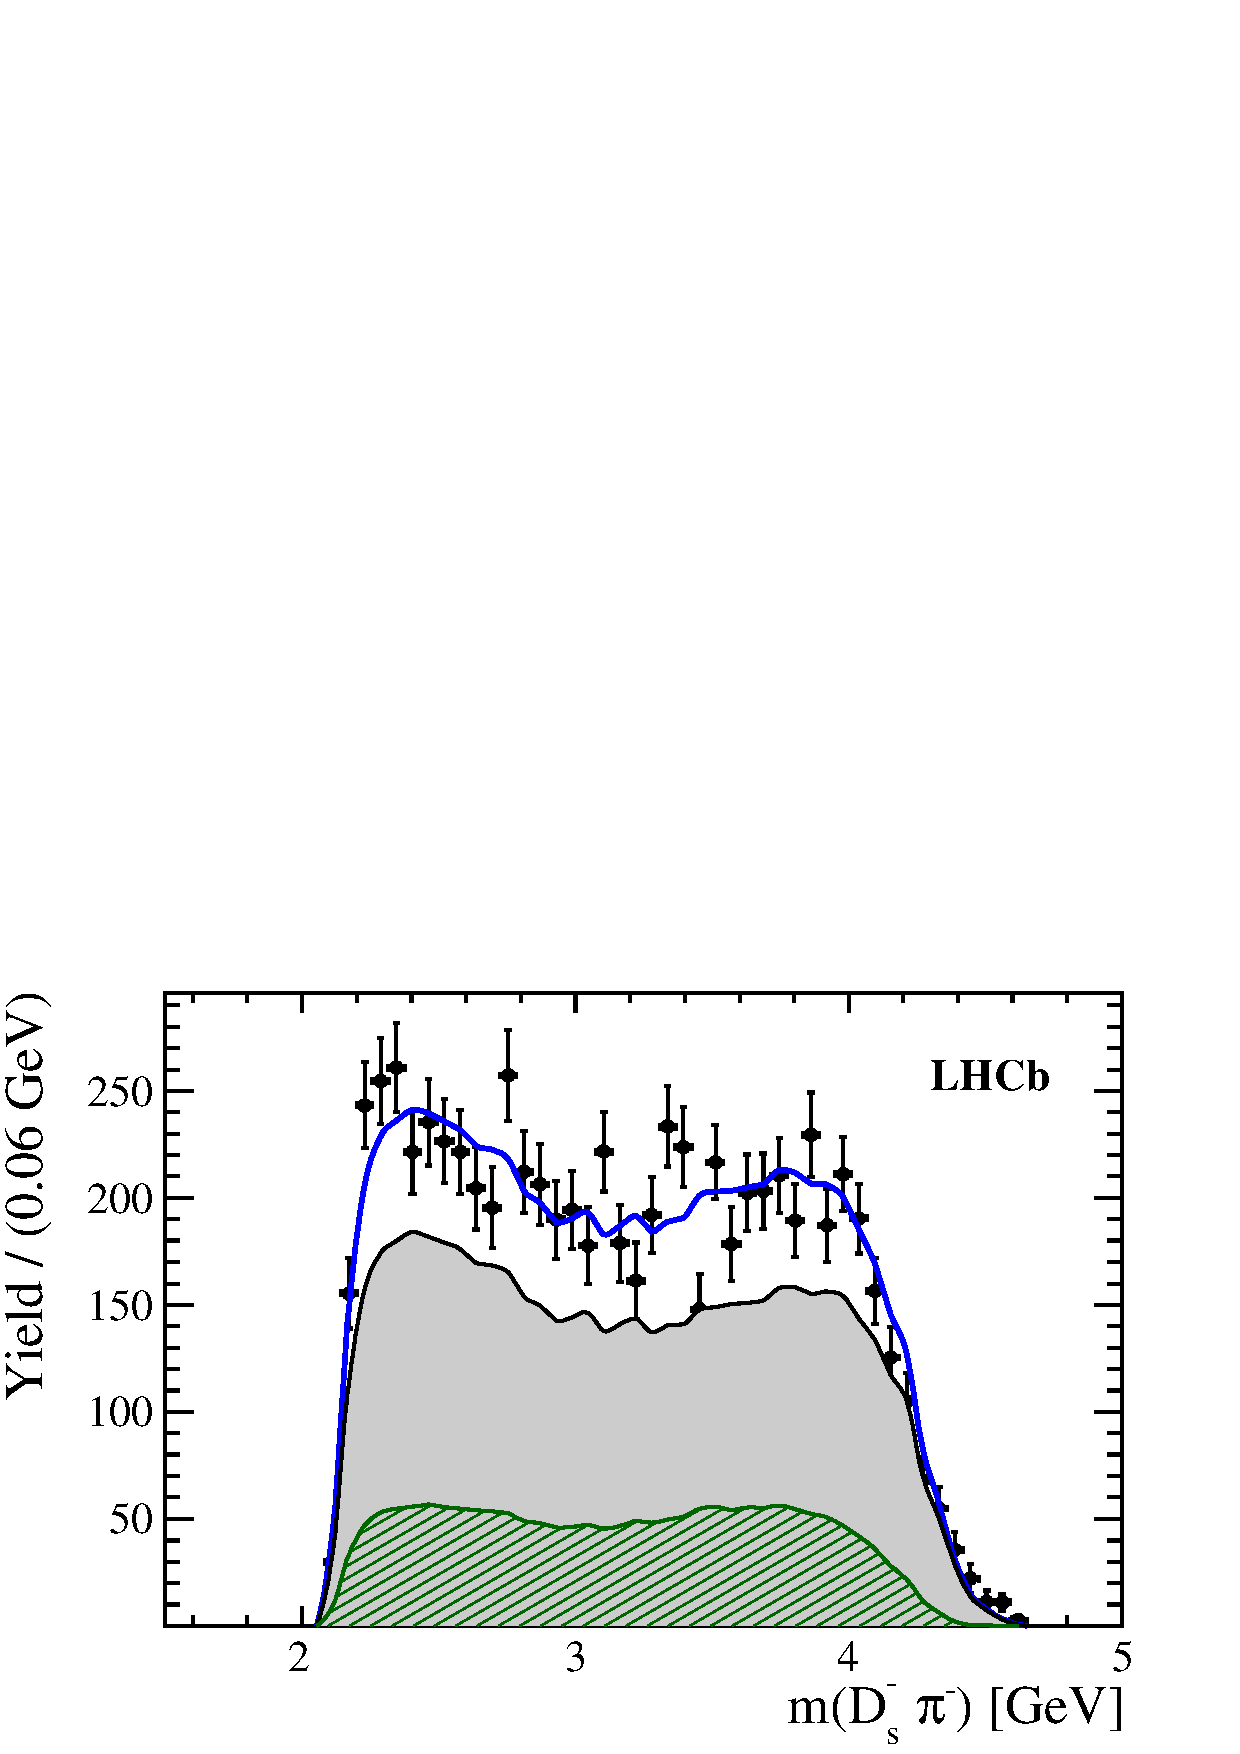
\includegraphics[width=0.32\textwidth, height = !]{figs/lassoFit/LASSO/m_Dspim_mod.pdf} 

		\includegraphics[width=0.32\textwidth, height = !]{figs/lassoFit/LASSO/m_Kpi_mod.pdf} 
		\includegraphics[width=0.32\textwidth, height = !]{figs/lassoFit/LASSO/m_pipi_mod.pdf} 
		\includegraphics[width=0.32\textwidth, height = !]{figs/lassoFit/LASSO/m_Dspi_mod.pdf} 
		
		\includegraphics[width=0.32\textwidth, height = !]{figs/lassoFit/LASSO/h_cosTheta_Kpi_mod.pdf} 
		\includegraphics[width=0.32\textwidth, height = !]{figs/lassoFit/LASSO/h_cosTheta_Dspi_mod.pdf} 
		\includegraphics[width=0.32\textwidth, height = !]{figs/lassoFit/LASSO/h_phi_Kpi_Dspi_mod.pdf} 

		\caption{} 		
\end{figure}	

\clearpage
\subsection{Results}

Table \ref{tab:lassoModel} 
lists the real and imaginary part of the complex amplitude coefficients $a_{i}$, 
obtained by fitting the LASSO model to the data,
along with the corresponding fit fractions. 
The letters in square brackets refer to the relative orbital angular momentum of the decay products. 
If no angular momentum is specified, the lowest angular momentum state consistent with angular momentum conservation and, where appropriate, parity conservation is used.
In order to provide implementation-independent measurements in addition to the complex coefficients $a_i$, we define two quantities. Firstly, the fit fractions
\begin{equation}
\label{eq:DefineFitFractions}
	F_{i} \equiv \frac{\int \left\vert   a_{i} \, A_{i}(\phsPoint) \right\vert^{2} \, \text{d}\Phi_{4} }
	{\int \left\vert  A_{\Dz}(\phsPoint) \right\vert^{2} \, \text{d}\Phi_{4}}, 
\end{equation}
which are a measure of the relative strength between the different transitions. Secondly, the interference fractions are given by
\begin{equation}
\label{eq:DefineInterferenceFractions}
	I_{ij} \equiv \frac{\int  2\,\Re[a_{i}a^*_{j} \, A_{i}(\phsPoint) A^*_{j}(\phsPoint) ] \, \text{d}\Phi_{4} }
	{\int \left\vert  A_{\Dz}(\phsPoint) \right\vert^{2} \, \text{d}\Phi_{4}} ,
\end{equation}
which measures the interference effects between amplitude pairs. Constructive interference leads to $I_{ij} > 0$, while destructive interference leads to $I_{ij} < 0$. Note that $\sum_i F_{i} + \sum_{j<k} I_{j,k} = 1$.
%The interference fractions are given in Appendix~\ref{a:interference}. 

Figure \ref{fig:baselineFit} shows the distributions of 
selected phase space observables, which demonstrate 
reasonable agreement between data and the fit model. 
We also project into the transversity basis to demonstrate good description of the overall angular structure in
Fig.~\ref{fig:baselineFit2}: 
The acoplanarity angle 
${\chi}$, is the angle between the two decay planes formed by 
the $\pi^+\pi^-$ combination with minimum invariant mass, ${\rm min}[m(\pi^+\pi^-)]$,  
and the remaining $\pip \pim$ combination
in the $D$ rest frame; boosting into the rest frames of the two-body systems defining these decay planes,
the two helicity variables 
are defined as the cosine of the angle, ${\theta}$, 
of each \pip\ momentum with the $D$ flight direction.

In order to quantify the quality of the fit in the five-dimensional phase space,
a \chisq value is determined by binning the data;
\begin{equation}
	\chi^{2} = \sum_{b=1}^{N_{\rm bins}} \frac{(N_{b}-N_{b}^{\rm exp})^{2}}{N_{b}^{\rm exp}},
\end{equation}
where $N_{b}$ is the number of data events in a given bin, 
$N_{b}^{\rm exp}$ is the event count predicted by the fitted PDF
and $N_{\rm bins}$ is the number of bins.
%The phase space is binned in terms of $min$
An adaptive binning
is used to ensure sufficient statistics in each bin for a robust $\chi^{2}$ calculation ~\cite{KKpipi}.
At least $25$ events per bin are required.
The number of degrees of freedom $\nu$, in an unbinned fit is bounded by $N_{\rm bins}-1$ and $(N_{\rm bins}- 1) - N_{\rm par}$, 
where $N_{\rm par}$ is the number of free fit parameters.
We use the \chisq value divided by $\nu = (N_{\rm bins}-1) - N_{\rm par}$ as a conservative estimate.
For the LASSO model, this 
amounts to $\chisq/\nu = 1.40$ %with $\nu = 221$,
indicating a decent fit quality.


\begin{figure}[h]
	\centering
		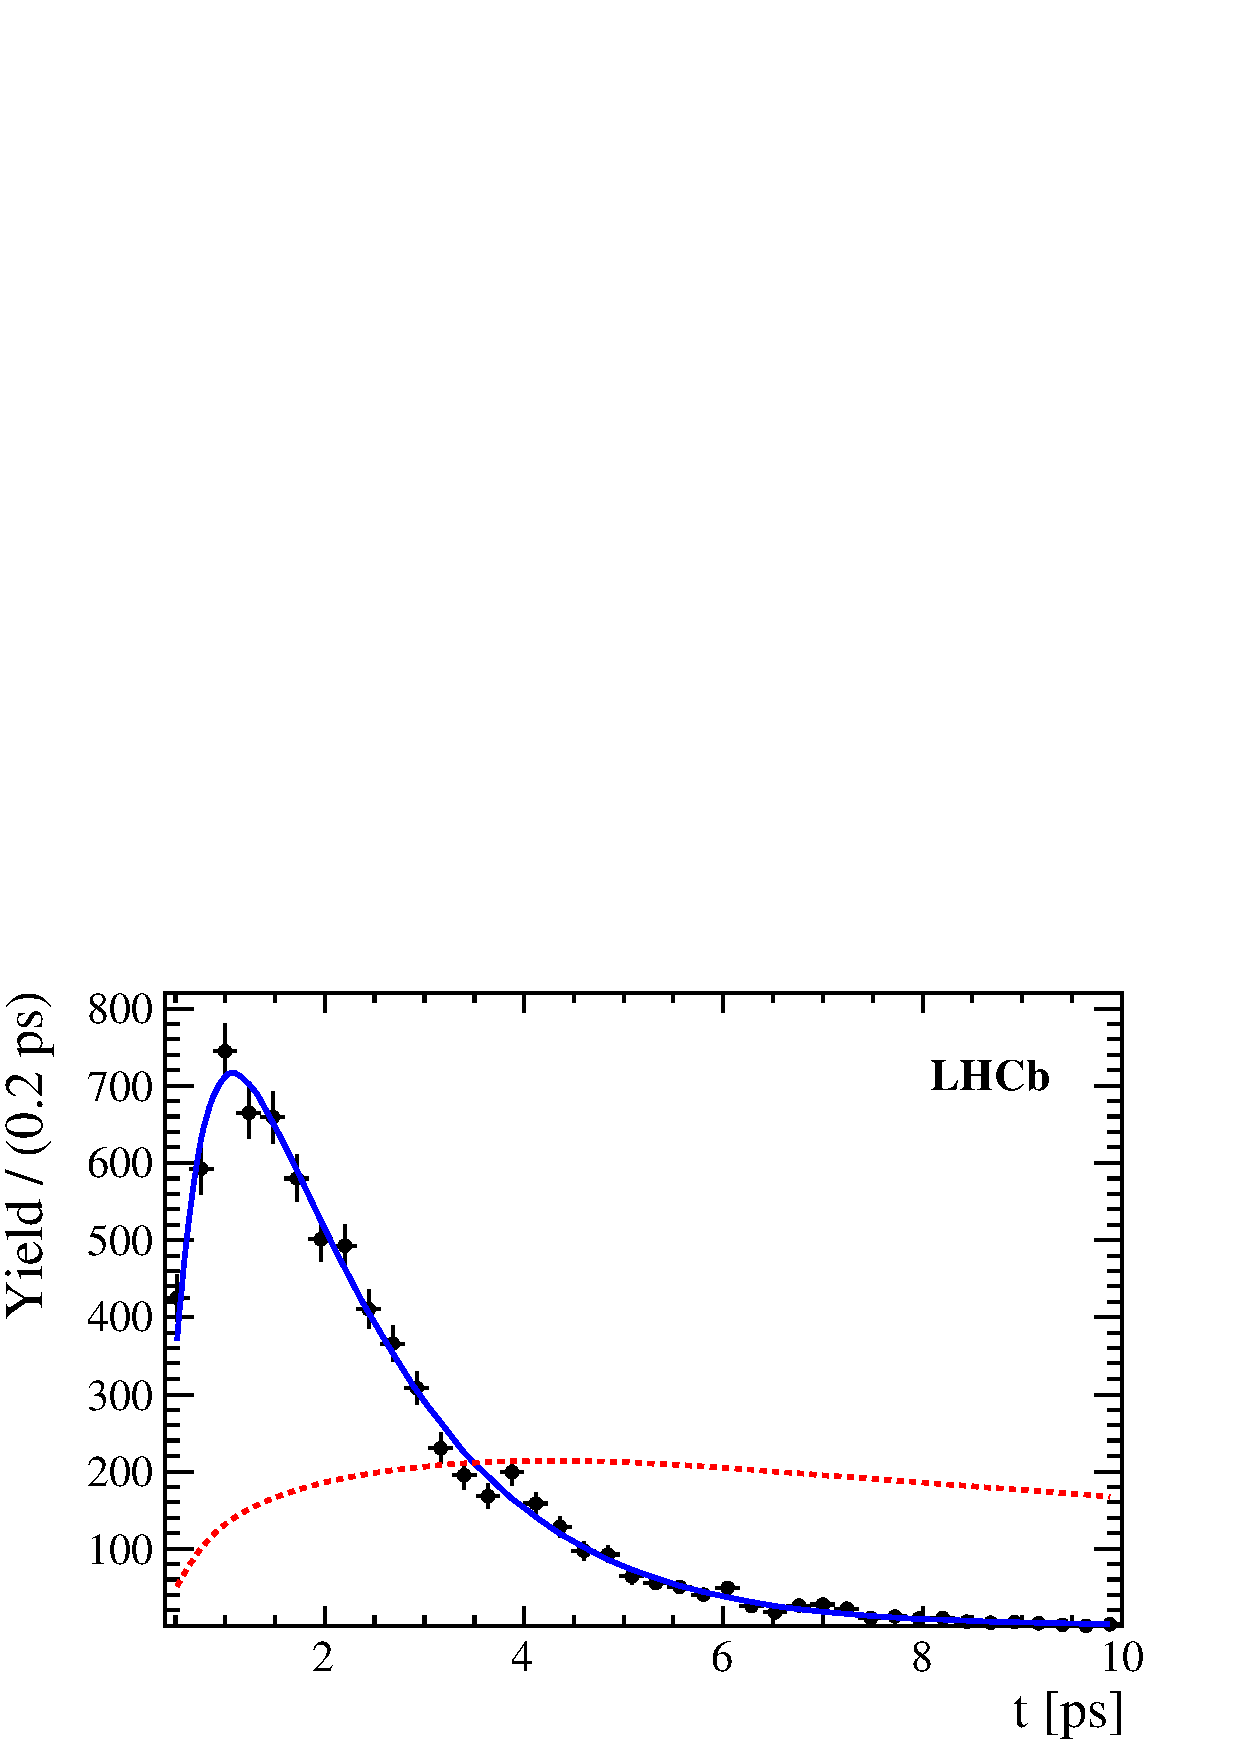
\includegraphics[width=0.3\textwidth, height = !]{figs/fullFit/signal/h_t.pdf} 
		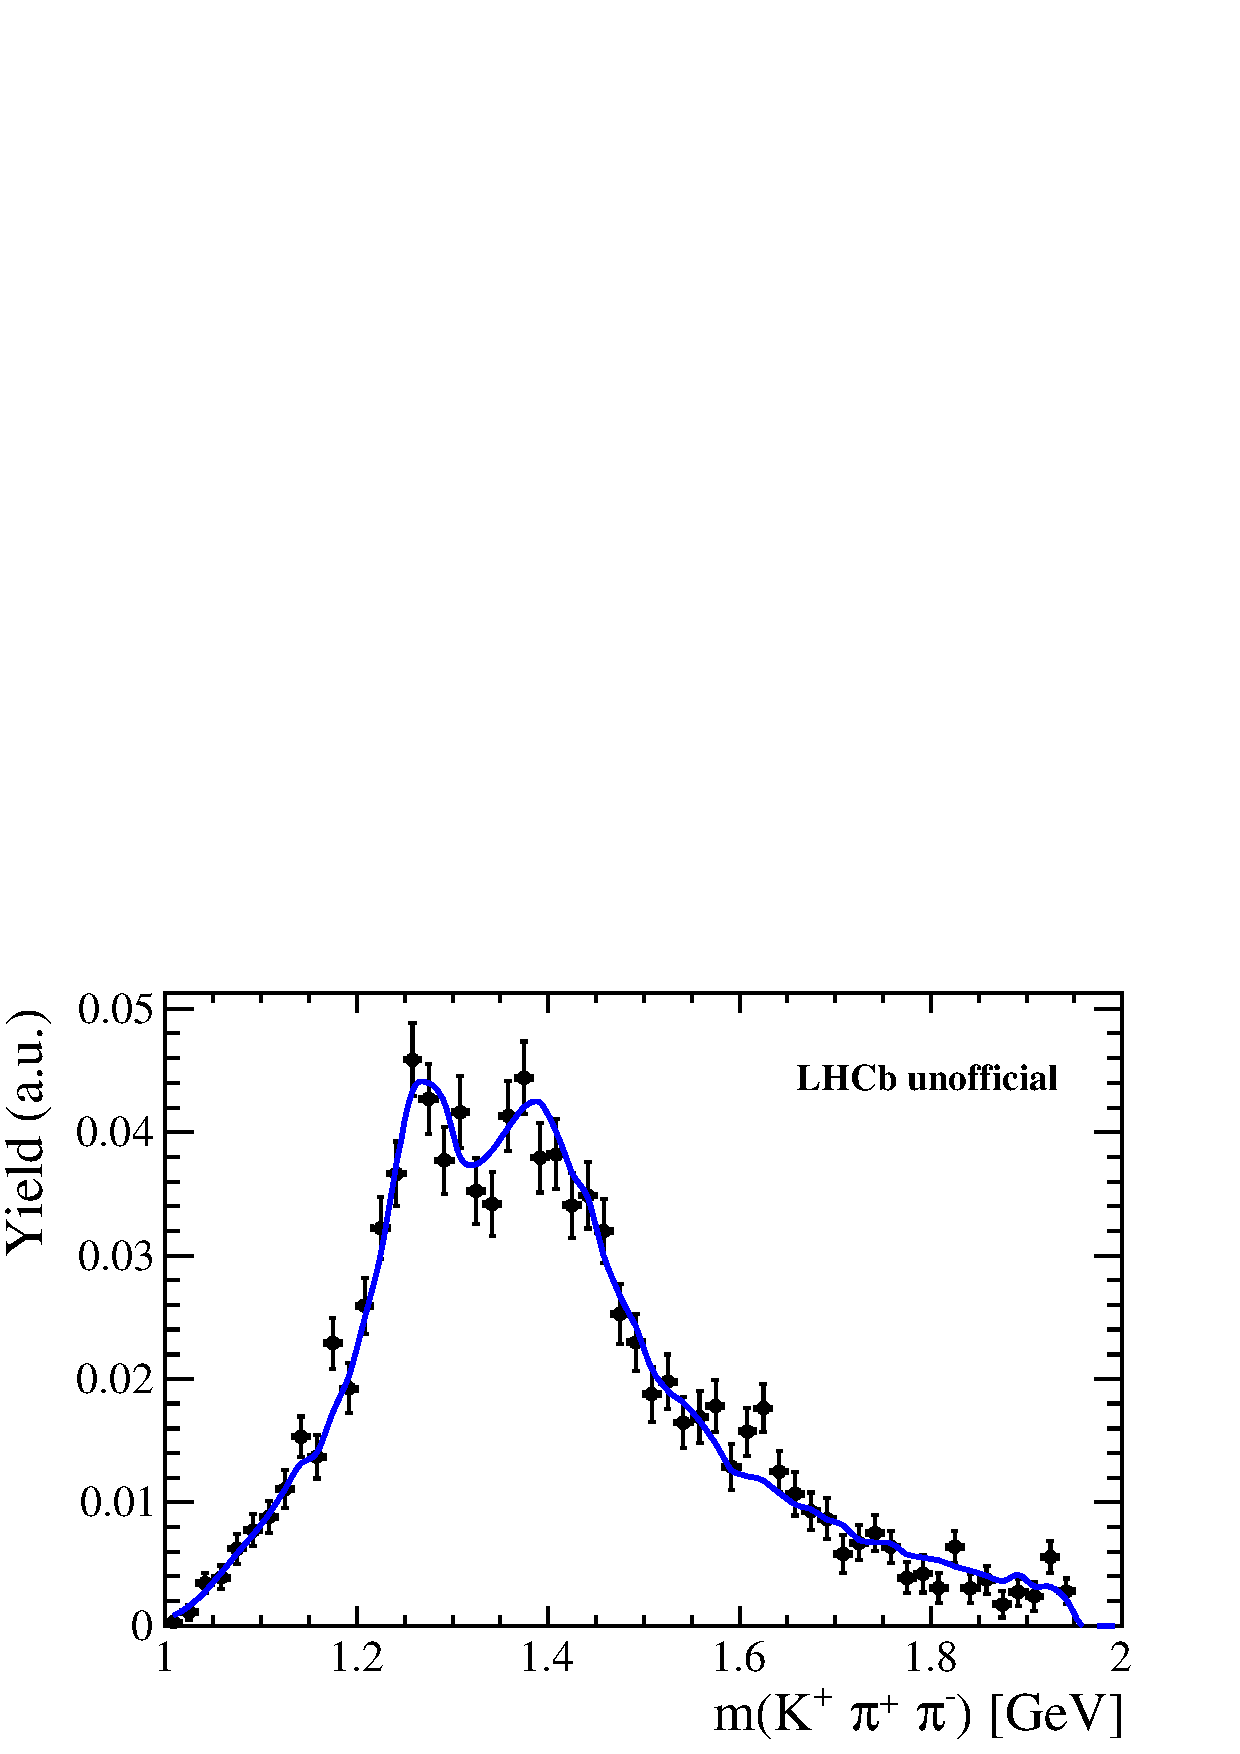
\includegraphics[width=0.3\textwidth, height = !]{figs/fullFit/signal/m_Kpipi.pdf} 
		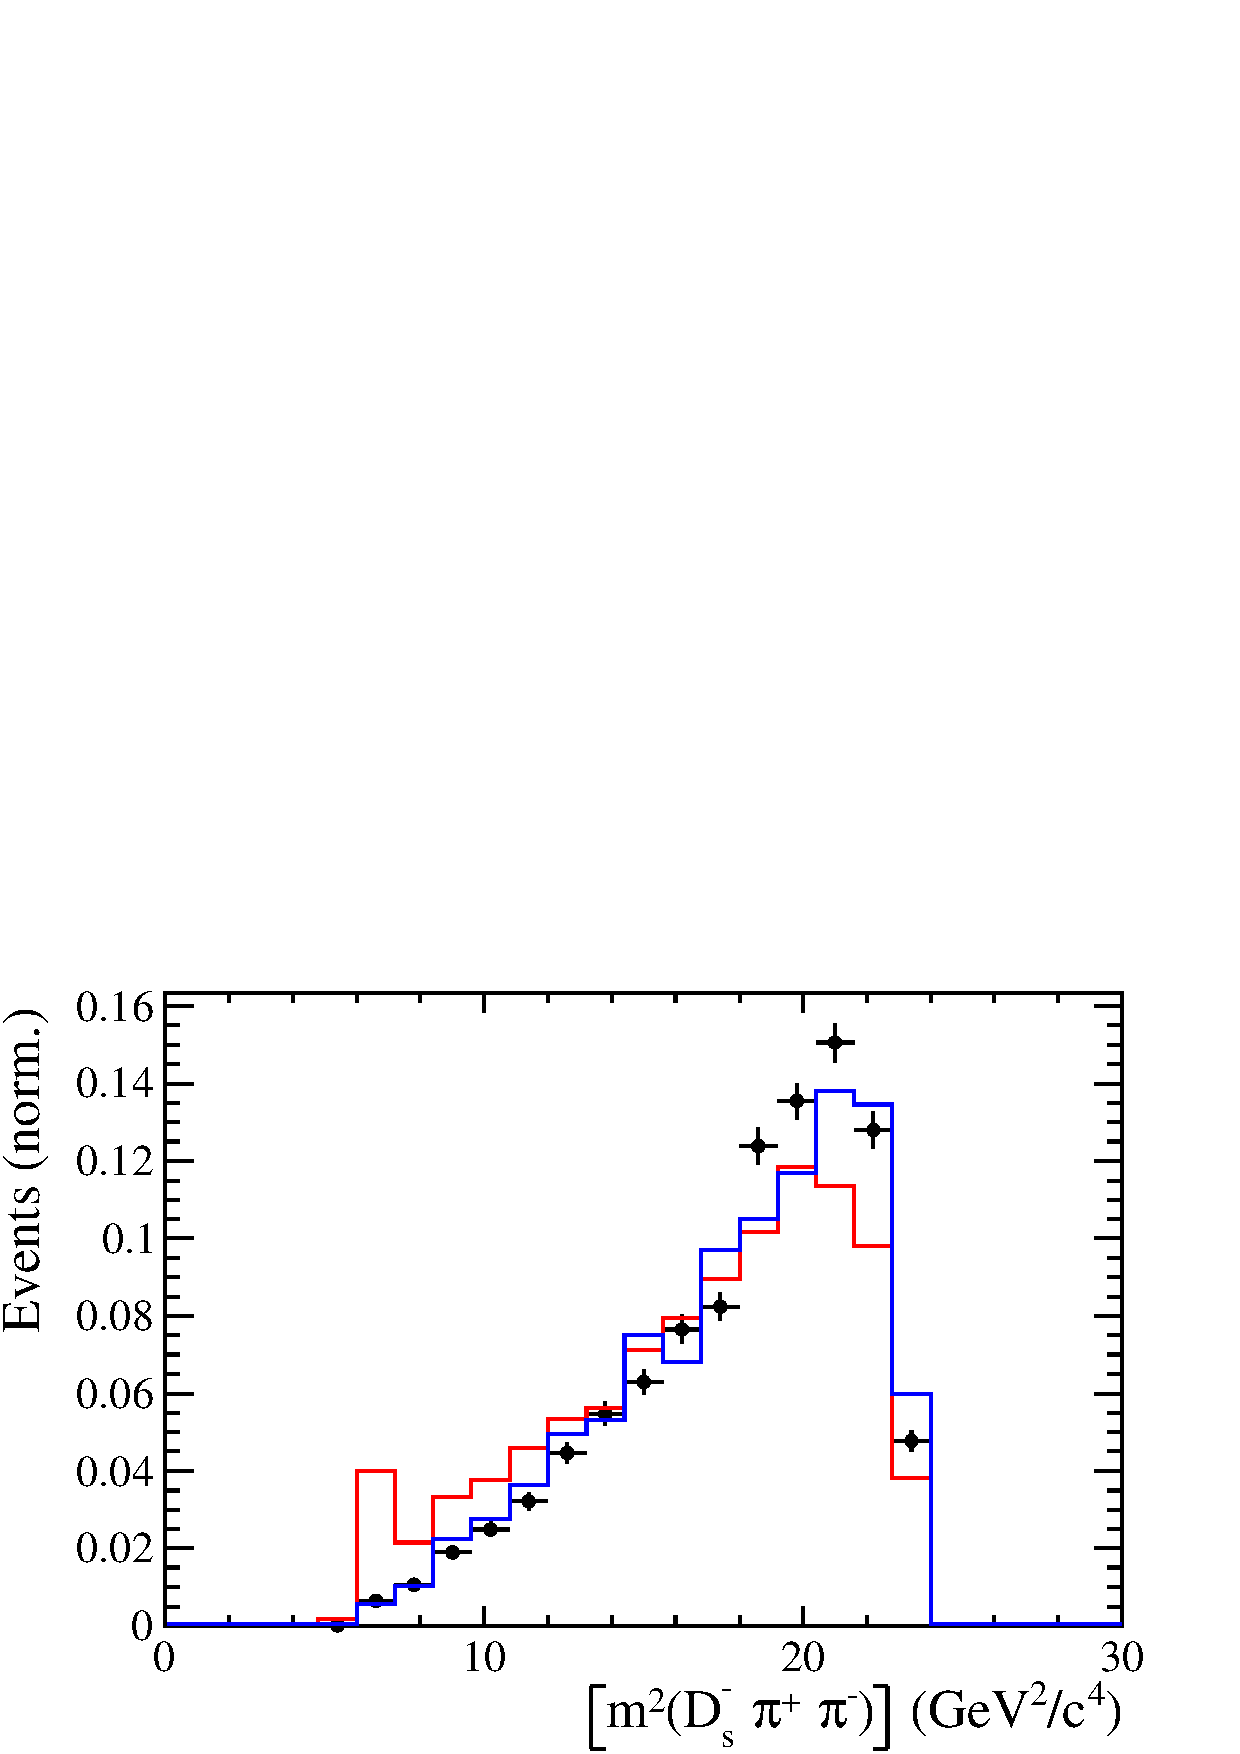
\includegraphics[width=0.3\textwidth, height = !]{figs/fullFit/signal/m_Dspipi.pdf} 

		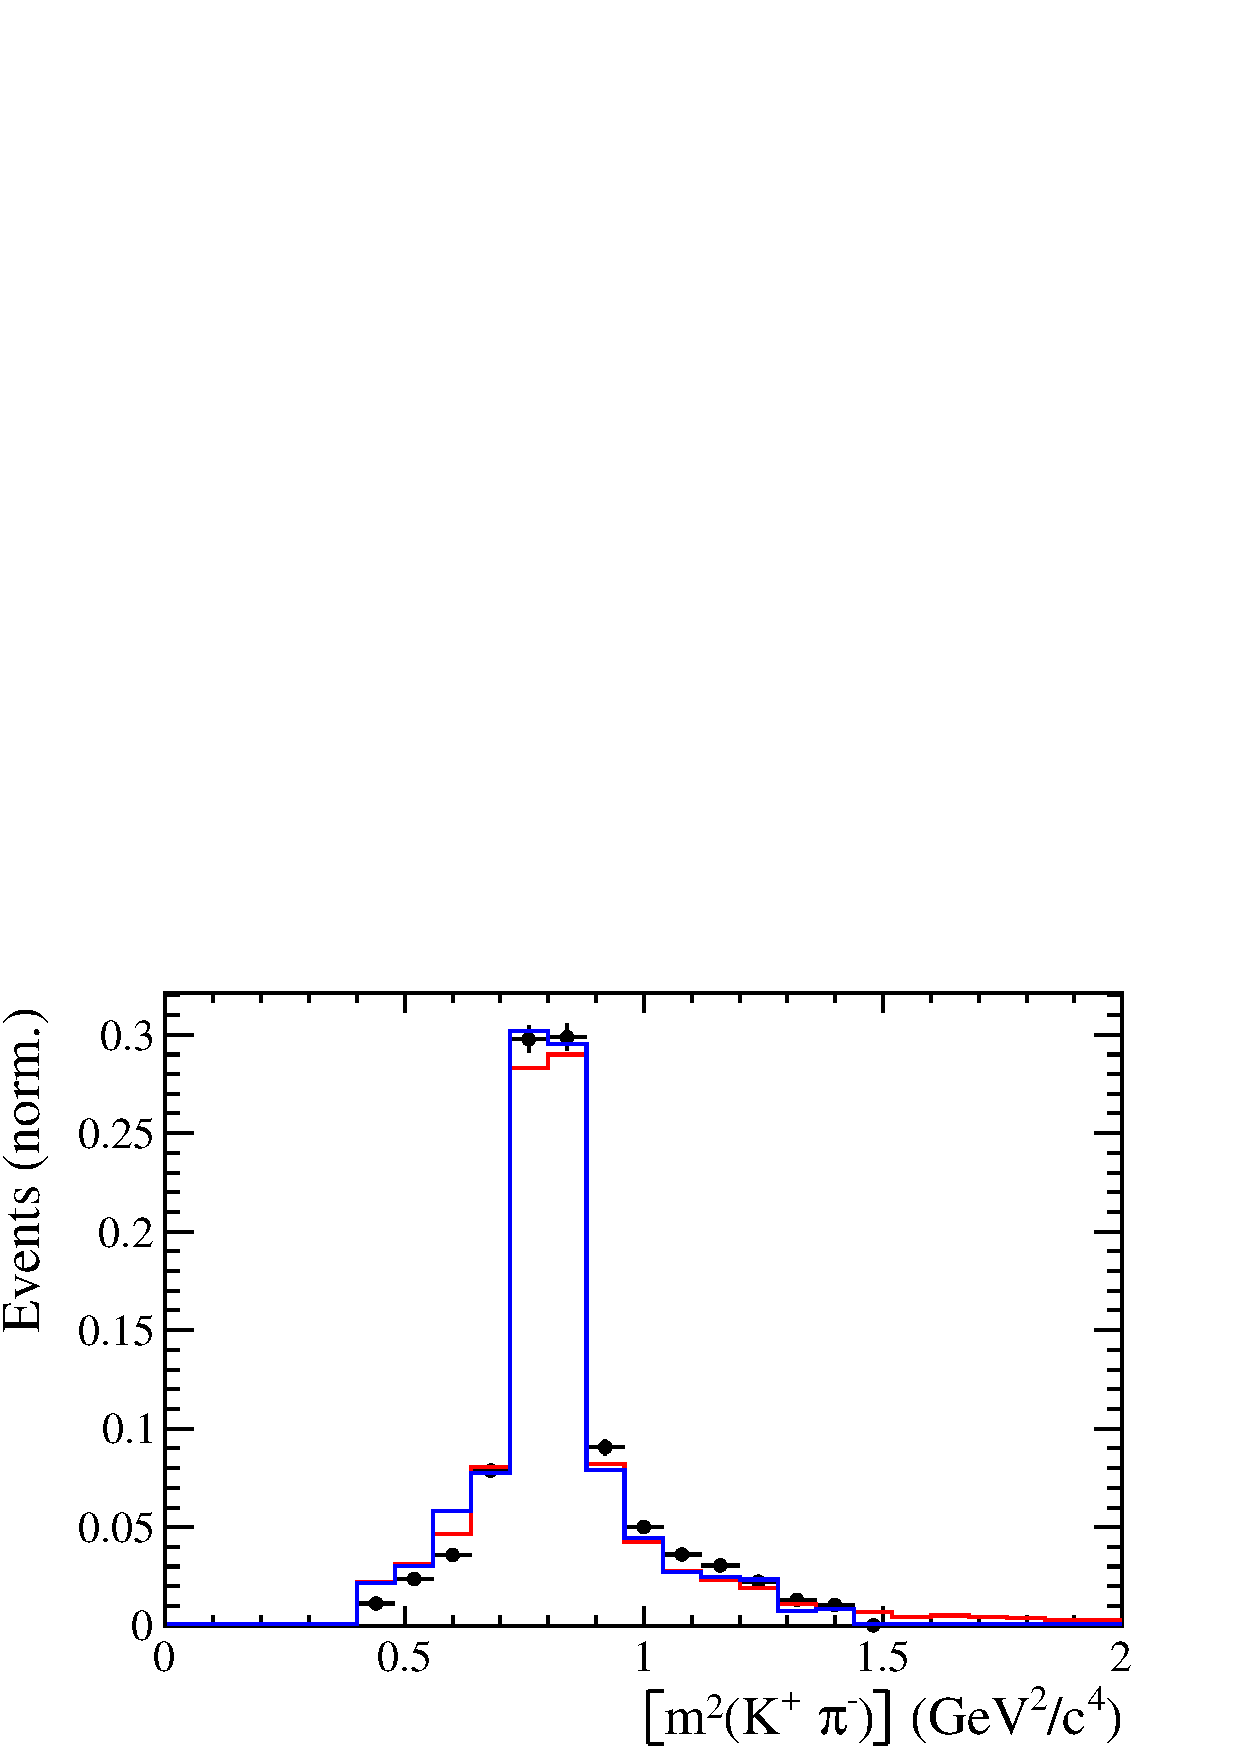
\includegraphics[width=0.3\textwidth, height = !]{figs/fullFit/signal/m_Kpi.pdf} 
		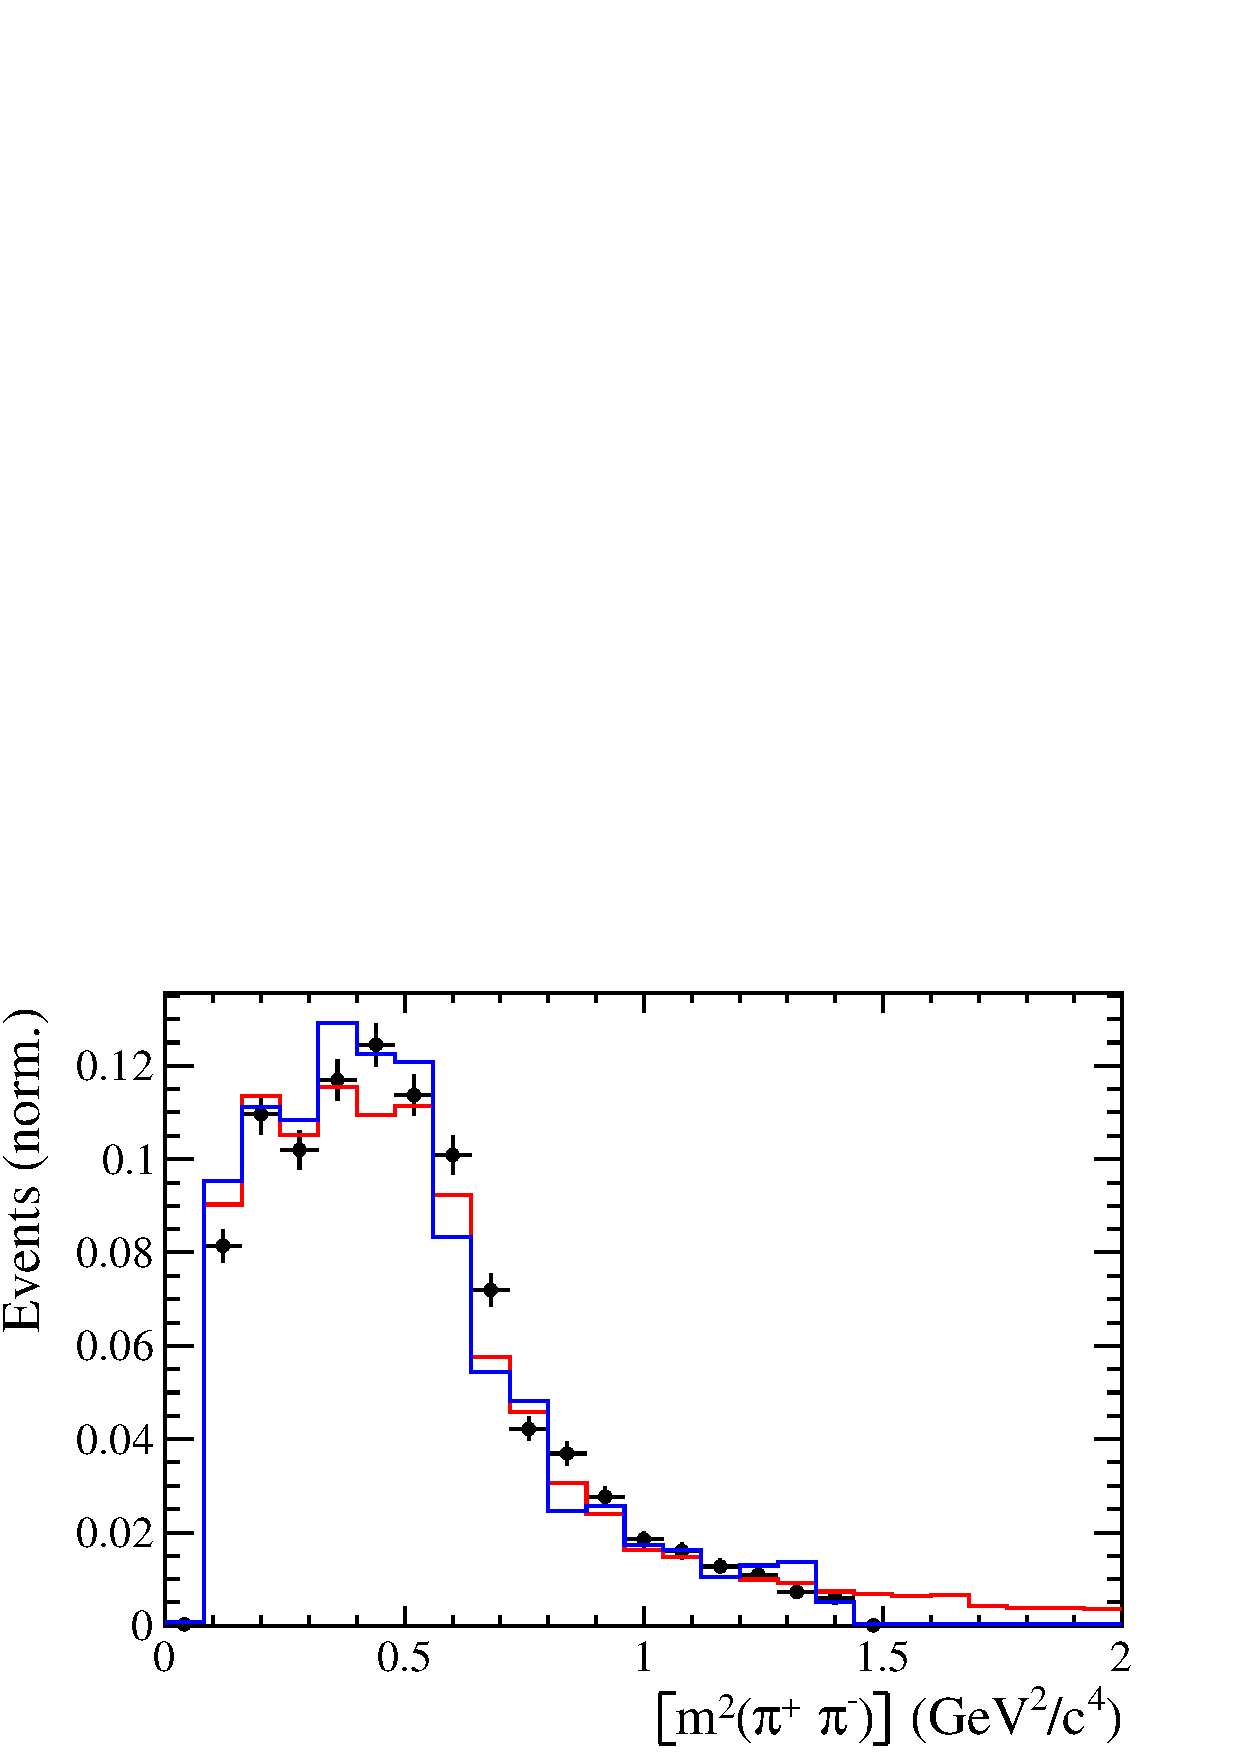
\includegraphics[width=0.3\textwidth, height = !]{figs/fullFit/signal/m_pipi.pdf} 
		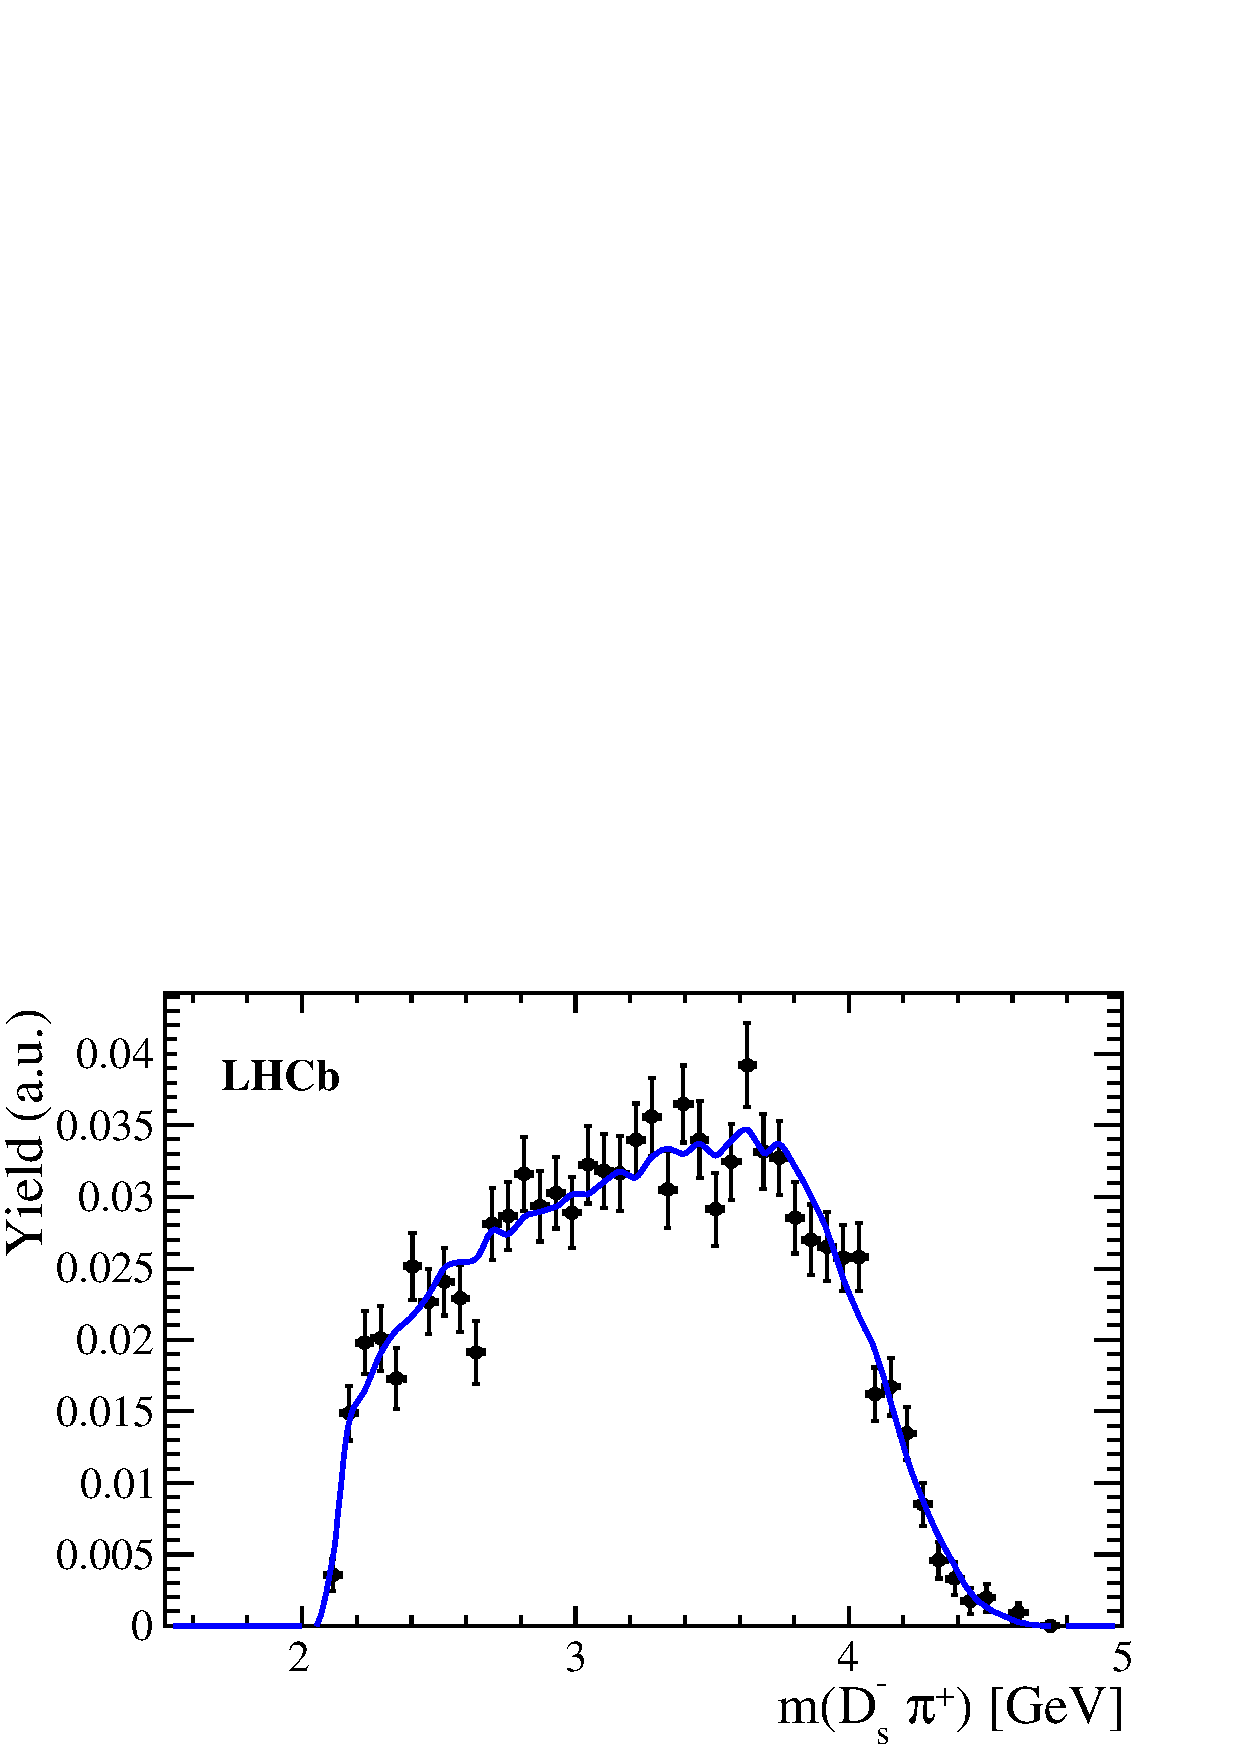
\includegraphics[width=0.3\textwidth, height = !]{figs/fullFit/signal/m_Dspi.pdf} 

		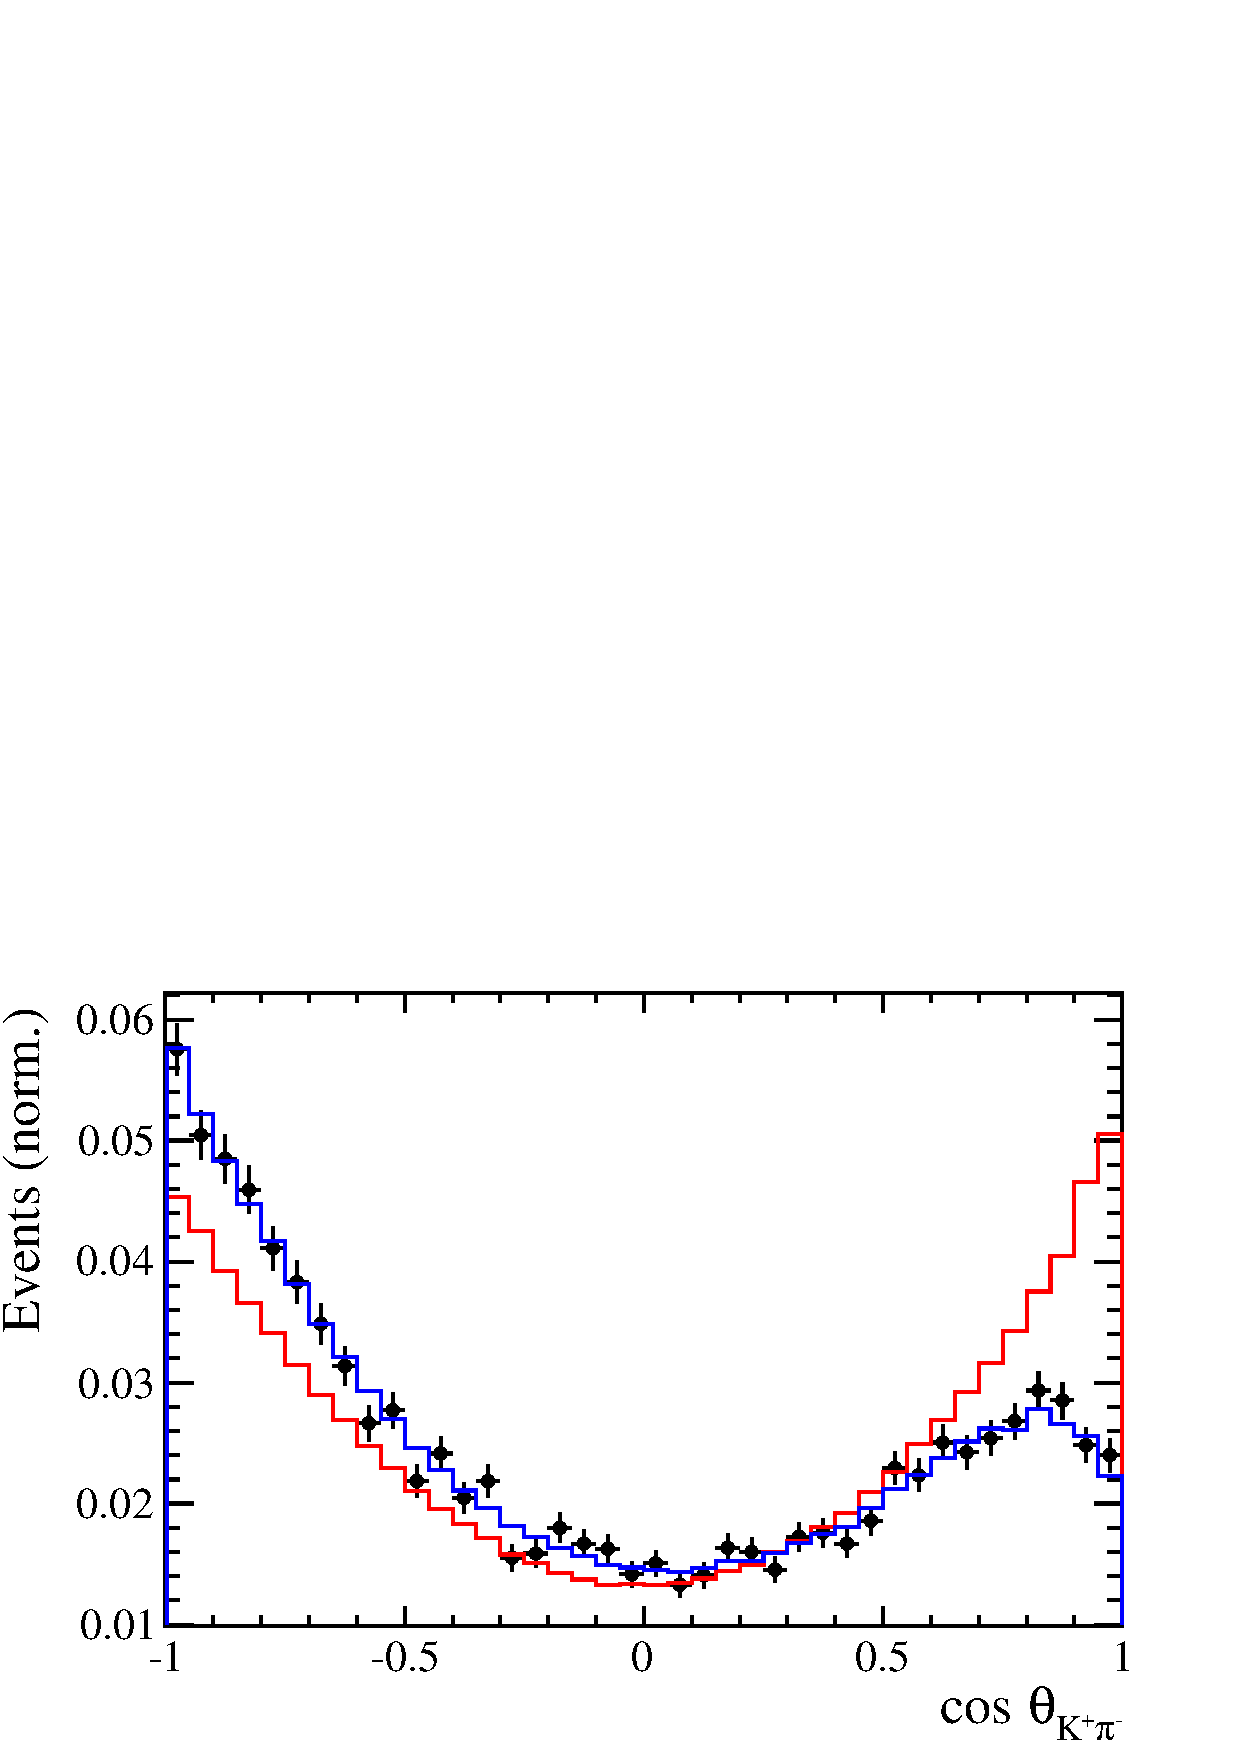
\includegraphics[width=0.3\textwidth, height = !]{figs/fullFit/signal/h_cosTheta_Kpi.pdf} 
		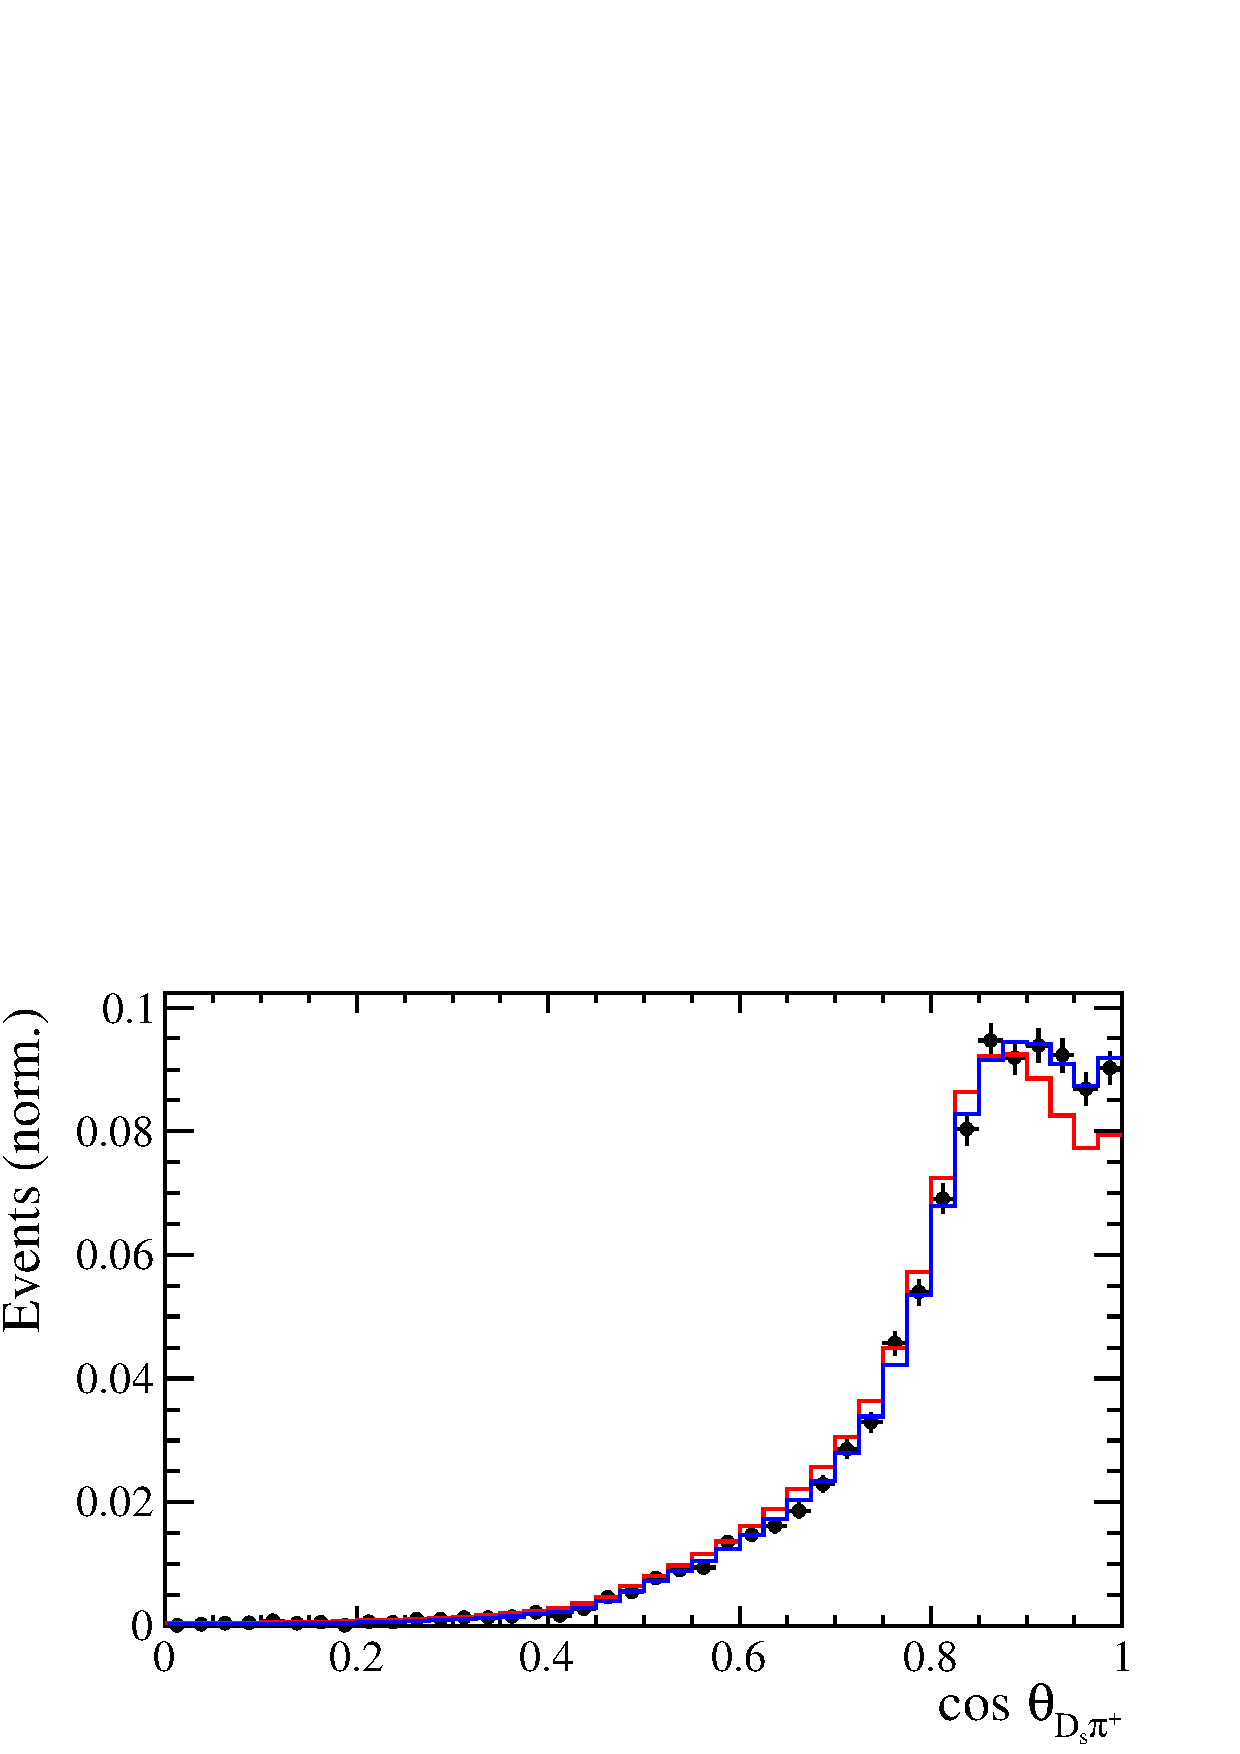
\includegraphics[width=0.3\textwidth, height = !]{figs/fullFit/signal/h_cosTheta_Dspi.pdf} 
		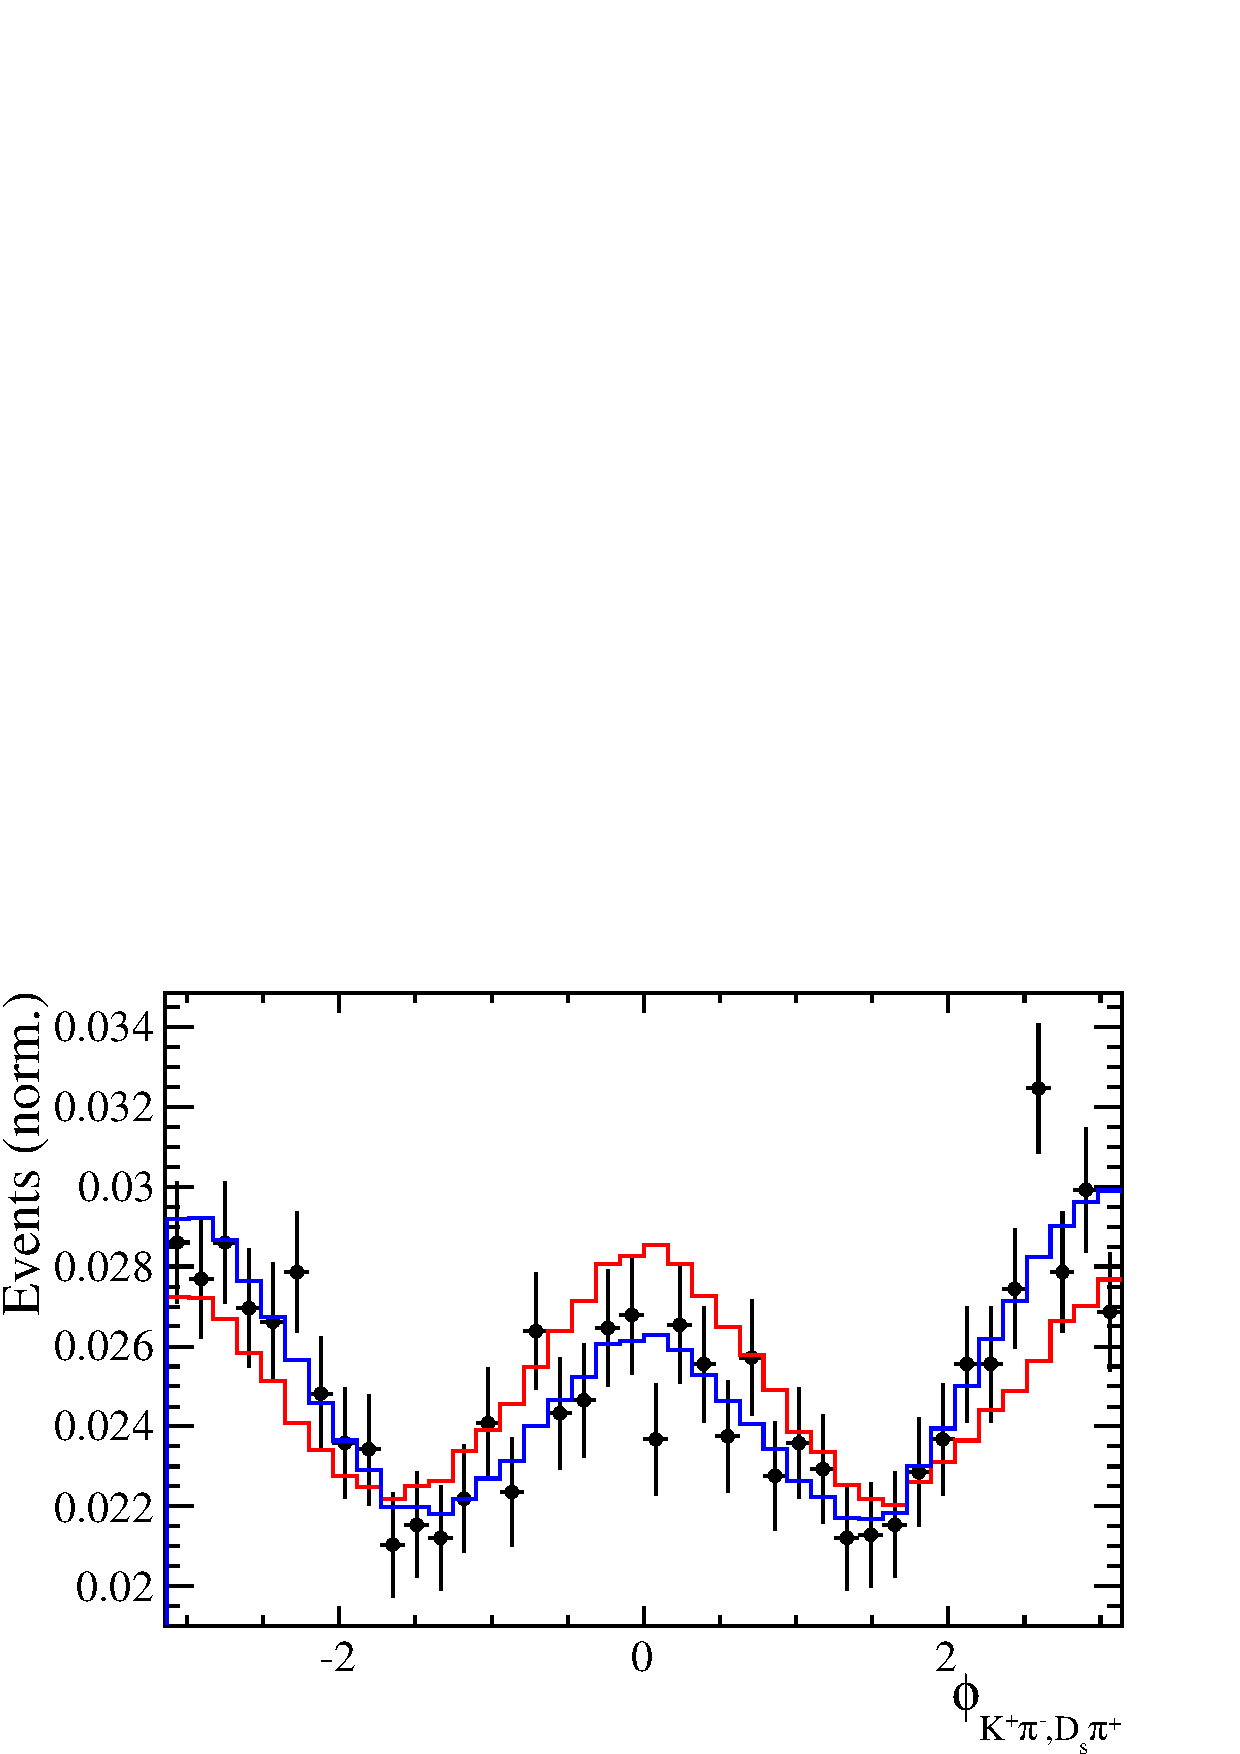
\includegraphics[width=0.3\textwidth, height = !]{figs/fullFit/signal/h_phi_Kpi_Dspi.pdf} 
		
%		\includegraphics[width=0.3\textwidth, height = !]{figs/fullFit/signal/m_Kpipi_mod.pdf} 
%		\includegraphics[width=0.3\textwidth, height = !]{figs/fullFit/signal/m_Dspipi_mod.pdf} 

%		\includegraphics[width=0.3\textwidth, height = !]{figs/fullFit/signal/m_Kpi_mod.pdf} 
%		\includegraphics[width=0.3\textwidth, height = !]{figs/fullFit/signal/m_pipi_mod.pdf} 
%		\includegraphics[width=0.3\textwidth, height = !]{figs/fullFit/signal/m_Dspi_mod.pdf} 
%
%		\includegraphics[width=0.3\textwidth, height = !]{figs/fullFit/signal/h_cosTheta_Kpi_mod.pdf} 
%		\includegraphics[width=0.3\textwidth, height = !]{figs/fullFit/signal/h_cosTheta_Dspi_mod.pdf} 
%		\includegraphics[width=0.3\textwidth, height = !]{figs/fullFit/signal/h_phi_Kpi_Dspi_mod.pdf} 

		\caption{} 		
\end{figure}	


\begin{table}[h]
\centering
\caption{
\small
Modulus and phases of the amplitudes contributing to $b \to c$ and $b \to u$ decays.
In case of multiple decay modes of three-body resonances, the amplitude coefficients are defined relative to the one listed first.
Additional fit parameters are listed below.
The first quoted uncertainty is statistical, while the second arises from systematic sources. 
The third uncertainty arises from the alternative models considered.
}
\resizebox{\linewidth}{!}{
	\renewcommand{\arraystretch}{1.5}
	\begin{tabular}{l c c c c } 
\hline
\hline
\multicolumn{1}{c}{Decay Channel} & \multicolumn{2}{c}{$A_{b \to c}$} & \multicolumn{2}{c}{$A_{b \to u}$}  \\ 
 & \multicolumn{1}{c}{$\vert a_i \vert$}  & \multicolumn{1}{c}{$arg(a_i) [\degrees]$}  & \multicolumn{1}{c}{$\vert a_i \vert$} & \multicolumn{1}{c}{$arg(a_i) [\degrees]$} \\ 
\hline
 $B_s \to D_s \, ( K_1(1270) \to K \, \rho(770) ) $ &  1.0 & 0.0 & 1.0 & 0.0  \\ 
$\phantom{B_s \to D_s \, (} K_1(1270) \to K^{*}(892) \, \pi \phantom{)} $ & 0.72 $\pm$ 0.11 $\pm$ 0.09 & 50.1 $\pm$ 8.4 $\pm$ 5.9 & &   \\ 
$\phantom{B_s \to D_s \, (} K_1(1270) \to K^{*}_{0}(1430) \, \pi \phantom{)} $ & 0.52 $\pm$ 0.04 $\pm$ 0.06 & 128.9 $\pm$ 5.0 $\pm$ 18.0 & &   \\ 
$B_s \to D_s \, ( K_1(1400) \to K^{*}(892) \, \pi ) $ & 1.98 $\pm$ 0.08 $\pm$ 0.19 & 10.5 $\pm$ 9.3 $\pm$ 6.2 & 0.74 $\pm$ 0.20 $\pm$ 0.16 & -64.3 $\pm$ 12.9 $\pm$ 13.2 \\ 
$B_s \to D_s \, ( K^{*}(1410) \to K^{*}(892) \, \pi ) $ & 1.14 $\pm$ 0.08 $\pm$ 0.09 & 55.0 $\pm$ 4.6 $\pm$ 5.1 &  &  \\ 
$\phantom{B_s \to D_s \, (} K^{*}(1410) \to K \, \rho(770) \phantom{)} $ & 0.63 $\pm$ 0.05 $\pm$ 0.04 & -164.1 $\pm$ 5.3 $\pm$ 3.2 & &   \\ 
$B_s \to D_s \, ( K(1460) \to K^{*}(892) \, \pi ) $ & & &0.87 $\pm$ 0.10 $\pm$ 0.10 & -96.3 $\pm$ 11.5 $\pm$ 11.3 \\ 
$B_s \to ( D_s \, \pi)_{P} \, \, K^{*}(892) $ & 0.72 $\pm$ 0.10 $\pm$ 0.13 & -17.2 $\pm$ 12.4 $\pm$ 13.0 & 1.13 $\pm$ 0.12 $\pm$ 0.15 & -16.8 $\pm$ 14.3 $\pm$ 16.8 \\ 
$B_s \to ( D_s \, K)_{P} \, \, \rho(770) $ & & &0.53 $\pm$ 0.08 $\pm$ 0.07 & 33.6 $\pm$ 10.6 $\pm$ 11.2 \\ 
\hline
\hline
\multicolumn{1}{c}{Fit parameter} & \multicolumn{4}{c}{Value}  \\ 
\hline
\multicolumn{1}{c}{$m_{K_1(1400)} \, [\text{MeV}]$} & \multicolumn{4}{c}{1397 $\pm$ 10 $\pm$ 5 $\pm$ 7} \\ 
\multicolumn{1}{c}{$\Gamma_{K_1(1400)} \, [\text{MeV}]$} & \multicolumn{4}{c}{205 $\pm$ 15 $\pm$ 11 $\pm$ 8} \\ 
\multicolumn{1}{c}{$m_{K^{*}(1410)} \, [\text{MeV}]$} & \multicolumn{4}{c}{1432 $\pm$ 10 $\pm$ 17 $\pm$ 8} \\ 
\multicolumn{1}{c}{$\Gamma_{K^{*}(1410)} \, [\text{MeV}]$} & \multicolumn{4}{c}{345 $\pm$ 25 $\pm$ 37 $\pm$ 17} \\ 
 \\ 
\multicolumn{1}{c}{$r$} & \multicolumn{4}{c}{0.50 $\pm$ 0.05 $\pm$ 0.03 $\pm$ 0.02} \\ 
\multicolumn{1}{c}{$\delta \, [\degrees]$} & \multicolumn{4}{c}{46 $\pm$ 14 $\pm$ 7 $\pm$ 8} \\ 
\multicolumn{1}{c}{$\gamma - 2 \beta_{s} \, [\degrees]$} & \multicolumn{4}{c}{61 $\pm$ 15 $\pm$ 6 $\pm$ 6} \\ 
\hline
\hline
\end{tabular}

}
\end{table}

\begin{table}[h]
\centering
\caption{
Fit fractions of the amplitudes contributing to $b \to c$ and $b \to u$ decays.
}
%\resizebox{\linewidth}{!}{
	\renewcommand{\arraystretch}{1.5}
	\begin{tabular}{l r r } 
\hline
\hline
\multicolumn{1}{c}{Decay Channel} & \multicolumn{1}{c}{$F_{b \to c} [\%]$} & \multicolumn{1}{c}{$F_{b \to u} [\%]$}  \\ 
\hline
$B_s \to D_s \, ( K_1(1270) \to K^{*}(892) \, \pi )$ & 6.3 $\pm$ 1.6 & 14.9 $\pm$ 4.5 \\ 
$B_s \to D_s \, ( K_1(1270) \to K \, \rho(770) )$ & 12.3 $\pm$ 1.4 & 29.1 $\pm$ 6.1 \\ 
$B_s \to D_s \, ( K_1(1270) \to K^{*}_{0}(1430) \, \pi )$ & 3.4 $\pm$ 0.5 & 8.0 $\pm$ 2.1 \\ 
$B_s \to D_s \, ( K_1(1400) \to K^{*}(892) \, \pi )$ & 48.3 $\pm$ 4.5 & 17.2 $\pm$ 8.6 \\ 
$B_s \to D_s \, ( K^{*}(1410) \to K^{*}(892) \, \pi )$ & 15.5 $\pm$ 1.0 &  \\ 
$B_s \to D_s \, ( K^{*}(1410) \to K \, \rho(770) )$ & 6.7 $\pm$ 0.6 &  \\ 
$B_s \to D_s \, ( K(1460) \to K^{*}(892) \, \pi )$ &  & 21.0 $\pm$ 4.6 \\ 
$B_s \to ( D_s \, \pi)_{P} \, \, K^{*}(892)$ & 6.8 $\pm$ 1.5 & 36.0 $\pm$ 8.0 \\ 
$B_s \to ( D_s \, K)_{P} \, \, \rho(770)$ &  & 9.7 $\pm$ 4.0 \\ 
\hline
$\text{Sum}$ & 99.3 $\pm$ 4.7 & 135.9 $\pm$ 12.9 \\ 
\hline
\hline
\end{tabular}

%}
\end{table}

